\ifx\PREAMBLE\undefined
\documentclass{report}
\usepackage[format = hang, font = bf]{caption}
% The following is needed in order to make the code compatible
% with both latex/dvips and pdflatex. Added for using UML generated by MetaUML.
\ifx\pdftexversion\undefined
\usepackage[dvips]{graphicx}
\else
\usepackage[pdftex]{graphicx}
\DeclareGraphicsRule{*}{mps}{*}{}
\fi
\usepackage{array}
\usepackage{amsmath}
\usepackage{amsthm}
\usepackage{mathtools}
\usepackage{boxedminipage}
\usepackage{listings}
\usepackage{makecell}%diagonal line in table
\usepackage{float}%allowing forceful figure[H]
\usepackage{xcolor}
\usepackage{amsfonts}%allowing \mathbb{R}
\usepackage{amssymb}
\usepackage{alltt}
\usepackage{algorithmicx}
\usepackage[chapter]{algorithm} 
%chapter option ensures that algorithms are numbered within each chapter rather than in the whole article
\usepackage[noend]{algpseudocode} %If end if, end procdeure, etc is expected to appear, remove the noend option
\usepackage{xspace}
\usepackage{color}
\usepackage{url}
\def\UrlBreaks{\do\A\do\B\do\C\do\D\do\E\do\F\do\G\do\H\do\I\do\J\do\K\do\L\do\M\do\N\do\O\do\P\do\Q\do\R\do\S\do\T\do\U\do\V\do\W\do\X\do\Y\do\Z\do\[\do\\\do\]\do\^\do\_\do\`\do\a\do\b\do\c\do\d\do\e\do\f\do\g\do\h\do\i\do\j\do\k\do\l\do\m\do\n\do\o\do\p\do\q\do\r\do\s\do\t\do\u\do\v\do\w\do\x\do\y\do\z\do\0\do\1\do\2\do\3\do\4\do\5\do\6\do\7\do\8\do\9\do\.\do\@\do\\\do\/\do\!\do\_\do\|\do\;\do\>\do\]\do\)\do\,\do\?\do\'\do+\do\=\do\#\do\-}
\usepackage[breaklinks = true]{hyperref}
\lstset{
language = C++, 
showspaces = false,
breaklines = true, 
tabsize = 2, 
numbers = left, 
extendedchars = false, 
basicstyle = {\ttfamily \footnotesize}, 
keywordstyle=\color{blue!70}, 
commentstyle=\color{gray}, 
frame=shadowbox, 
rulesepcolor=\color{red!20!green!20!blue!20}, 
numberstyle={\color[RGB]{0,192,192}}, 
moredelim=[is][\underbar]{_}{_}
}
\mathchardef\myhyphen="2D
% switch-case environment definitions
\algblock{switch}{endswitch} 
\algblock{case}{endcase}
%\algrenewtext{endswitch}{\textbf{end switch}} %If end switch is expected to appear, uncomment this line.
\algtext*{endswitch} % Make end switch disappear
\algtext*{endcase}
\algnewcommand\algorithmicinput{\textbf{input:}}
\algnewcommand\Input{\item[\algorithmicinput]}
\algnewcommand\algorithmicoutput{\textbf{output:}}
\algnewcommand\Output{\item[\algorithmicoutput]}
\allowdisplaybreaks
\newtheorem{theorem}{Theorem}[chapter]
\newtheorem{corollary}[theorem]{Corollary}
\newtheorem{lemma}[theorem]{Lemma}
\newtheorem{definition}{Definition}[chapter]
\begin{document}
\fi
\chapter{Graph Algorithms}
\textbf{Graphs represent pairwise relationships amongst a set of objects}. The objects are called vertices or nodes. The relationships are called edges or arcs, each connecting a pair of vertices. An edge can be directed or undirected. The set of vertices and the set of edges are noted respectively as $V$ and $E$. Graph is a concept heavily used in reality. Road networks, the web, social networks, precedence constraints are all examples of graphs.

A connected graph composed of $n$ vertices with no parallel edges has at least $n-1$ and at most $n(n-1)/2$ edges. Let $m$ represent the number of edges. In most applications, $m$ is $\Omega(n)$ and $O(n^2)$. If $m$ is $O(n)$ or close to it, the graph is called a sparse graph, while if $m$ is closer to $O(n^2)$, it's called a dense graph. Yet their delimitation is not strictly clear. 
\section{Representation}
\subsection{Adjacent Matrix}
An undirected graph $G$ with $n$ vertices and no parallel edges can be represented by an $n\times n$ 0-1 matrix $A$. $A_{ij}=1$ when and only when $G$ has an $i-j$ edge. Variants of this representation can easily accommodate parallel edges, weighted edges: just let $A_{ij}$ represent the number of parallel edges or the weight of the edge. For directed graphs, $i\rightarrow j$ can be represented by $A_{ij}=1$ and $A_{ji}=-1$.

Adjacent matrix representation requires $\Theta(n^2)$ space. For a dense graph this is fine, but for a sparse graph it is wasteful. 
\subsection{Adjacent Lists}
The adjacent lists representation is composed of 4 ingredients:
\begin{itemize}
\item Array/List of vertices. $\Theta(n)$ space.
\item Array/List of edges. $\Theta(m)$ space.
\item Each edge points to its end points. $\Theta(m)$ space.
\item Each vertex points to edges incident on it. $\Theta(m)$ space.
\end{itemize}
Adjacent lists representation requires $\Theta(n+m)$ space. 

The choice between the two representations depends on the density of the graph and operations to take. We will mainly use adjacent lists in this chapter.
\section{Minimum Cut}
\subsection{Definition}
\begin{definition}
A cut of a graph ($V,E$) is a partition of $V$ into two non-empty sets $A$ and $B$.
\end{definition}
A graph with $n$ vertices has $2^n-2$ possible cuts. 
\begin{definition}
The crossing edges of a cut($A,B$) are those with 
\begin{itemize}
\item one endpoint in $A$ and the other in $B$, for undirected graphs;
\item tail in $A$ and head in $B$, for directed graphs.
\end{itemize}
\end{definition}
We will try to solve the minimum cut problem:
\begin{description}
\item[Input]An undirected graph $G=(V,E)$ in which parallel edges are allowed.
\item[Output]A cut $(A,B)$ with minimum number of crossing edges.
\end{description}
A lot of problems in reality can be reduced to a minimum cut problems:
\begin{itemize}
\item Identify weakness point of physical networks;
\item Community detection in social networks;
\item Image segmentation.
\end{itemize}
\subsection{Random Contraction Algorithm}
Algorithm \ref{randomcontraction} provides a random approach to find a cut. 
\begin{algorithm}[ht]
\caption{Random Contraction}\label{randomcontraction}
\begin{algorithmic}[1]
\Input\Statex{An undirected graph $G=(V,E)$ in which parallel edges are allowed.}
\Output\Statex{A cut $(A,B)$ with minimum number of crossing edges}
\While{There are more than 2 vertices left}
\State{Pick a remaining edge $(u,v)$ randomly}\label{randomselection}
\State{Merge(or contract) $u,v$ into a single vertex}
\State{Remove self-loops}
\EndWhile
\State{Return cut represented by 2 final vertices}
\end{algorithmic}
\end{algorithm}
\subsection{Probability of Correctness}
Algorithm \ref{randomcontraction} is not guaranteed to always return a minimum cut. We have to iterate the whole algorithm multiple times and choose the cut with minimum number of crossing edges obtained during the process. In order to estimate the number of iterations needed, we will calculate the probability that a specific minimum cut $(A,B)$ is returned in one iteration.

If one of the crossing edges of $(A,B)$ is selected in step \ref{randomselection}, the minimum cut cannot be returned. If there are $k$ crossing edges in $(A,B)$, the probability that a crossing edge is selected at the first iteration is $k/m$. The number of edges decrease by an indefinite number at each iteration, while the number of vertices decrease by exactly 1 each time. Thus it is preferable to express the probability in terms of $n$ instead of $m$.

Each vertex $v$ is related to a cut $({v},V-{v})$. The number of crossing edges of this cut is the number of edges incident on $v$, i.e. the degree of $v$. Considering the definition of minimum cut, this number must be larger than $k$. We also know the sum of the degrees of all vertices: $\sum\limits_{v}degree(v)=2m$. Thus we have $2m=\sum\limits_{v}degree(v)\geq kn$. Hence the probability that a crossing edge is not selected at the first iteration in step \ref{randomselection} is $$1-k/m\geq 2/n.$$

At the second iteration, the same argument still holds. Let $m'$ represent the number of remaining edges after the first iteration. We have $2m'=\sum\limits_{v}degree(v)\geq k(n-1)$. Thus the probability that a crossing edge is selected at the 2nd iteration under the condition that no crossing edge was selected at the 1st iteration is $$1-k/m'\geq 2/(n-1)$$.

The same argument continues further until the last iteration, i.e. the $(n-2)^{th}$ iteration. Finally, the probability that no crossing edge is selected in the whole process, thus resulting in the minimum cut $(A,B)$ is
\begin{align*}
P(A,B)&\geq\left(1-\frac{2}{n}\right)\left(1-\frac{2}{n-1}\right)\cdots\left(1-\frac{2}{n-(n-3)}\right)\\
&=\frac{(n-2)\cdot(n-3)\cdots 2\cdot 1}{n\cdot(n-1)\cdots 4\cdot 3}\\
&=\frac{2}{n(n-1)}>\frac{1}{n^2}.
\end{align*}
The probability seems small, but it already makes great advancement when compared with brute-force method, in which case the probability to obtain $(A,B)$ in an iteration is $\frac{1}{2^n}$.

After $N$ iterations, the probability that $(A,B)$ has not been found is 
\begin{equation*}
P(not\:found)<\left(1-\frac{1}{n^2}\right)^N\leq e^{-\frac{N}{n^2}}.
\end{equation*}
If $N=n^2$, the probability is smaller than $1/e$. If $N=n^2\ln n$, it is smaller than $1/n$. 
\subsection{Number of Minimum Cuts}
A graph can have multiple minimum cuts. For example, a tree with $n$ vertices has $n-1$ minimum cuts. We would like to find the largest number of minimum cuts that a graph with $n$ vertices can have.
\begin{theorem}
A graph with $n$ vertices can have at most $\binom{n}{2}$ minimum cuts.
\end{theorem}
\begin{proof}
Consider the graph in which the $n$ vertices form a circle. Removing any two edges results in a minimum cut. Thus in total it has $\binom{n}{2}$ minimum cuts. The rest of the proof aims at proving that a graph with $n$ vertices cannot have more minimum cuts.

Recall that the probability for Algorithm \ref{randomcontraction} to return a specific minimum cut is bigger than $\frac{2}{n(n-1)}$. Suppose there are $k$ minimum cuts. The events ``Algorithm \ref{randomcontraction} returns minimum cut $C_i$'' and  ``Algorithm \ref{randomcontraction} returns minimum cut $C_j$'' are disjoint events when $i\neq j$. Thus we have 
$$1\geq P(\text{return a minimum cut})\geq\frac{2k}{n(n-1)}.$$
Therefore, 
$$k\leq \frac{n(n-1)}{2}=\binom{n}{2}.$$
\end{proof}
\section{Breadth First Search}
Graph search is widely used for various purposes:
\begin{itemize}
\item Check if a network is connected;
\item Find shortest paths, e.g. for driving navigation, or formulating a plan;
\item Calculate connected components.
\item $\dots$
\end{itemize}
We will introduce a few fast algorithms based on graph search. Graph search usually starts from a source vertex. When searching the graph, we want to find everything that is findable, i.e. every vertex reachable from the source via a path. Moreover, we never explore anything twice. In terms of running time, our goal is $O(m+n).$ 

BFS explores the nodes of a graph in layers. Nodes with the same distances from the source are in the same layer. It can be used to compute shortest paths of graphs, and to compute connected components of undirected graphs. It guarantees $O(m+n)$ running time. The general pattern of BFS is shown in Algorithm \ref{bfs}.
\begin{algorithm}[ht]
\caption{Breadth First Search(BFS)}\label{bfs}
\begin{algorithmic}[1]
\Input\Statex{Graph $G$ with all vertices unexplored}
\Statex{Source vertex $s$}
\Output\Statex{$G$ with all vertices reachable from $s$ explored.}
\State{Mark $s$ as explored.}
\State{Let $Q$ = queue initialized with $s$}
\While{$Q\neq\emptyset$}
\State{Remove first element $v$ of $Q$}
\For{each edge $(v,w)$}
\If{$w$ is unexplored}
\State{Mark $w$ as explored}
\State{Add $w$ to $Q$}
\EndIf
\EndFor
\EndWhile 
\end{algorithmic}
\end{algorithm}

At the end of BFS, the fact that a node $v$ is explored means the existence of a path from $s$ to $v$. 
\subsection{Shortest Path}
Algorithm \ref{shortestpath} calculates the shortest path from $s$ to any vertex reachable from $s$.
\begin{algorithm}[ht]
\caption{Shortest Path - BFS}\label{shortestpath}
\begin{algorithmic}[1]
\Input\Statex{Graph $G$ with all vertices unexplored}
\Statex{Source vertex $s$}
\Output\Statex{$dist(v)$ for any vertex $v$, i.e. min number of edges on a path from $s$ to $v$}
\State{Initialize $dist(v)=\left\{\begin{array}{rl}0,&if(v==s)\\+\infty,&if(v\neq s)\end{array}\right.$}
\State{Mark $s$ as explored.}
\State{Let $Q$ = queue initialized with $s$}
\While{$Q\neq\emptyset$}
\State{Remove first element $v$ of $Q$}
\For{each edge $(v,w)$}
\If{$w$ is unexplored}
\State{Mark $w$ as explored}
\State{$dist(w)=dist(v)+1$}
\State{Add $w$ to $Q$}
\EndIf
\EndFor
\EndWhile 
\end{algorithmic}
\end{algorithm}

After the algorithm terminates, $dist(v)=i$ means that $v$ is in the $i^{th}$ layer and that the shortest path connecting $s$ and $v$ has $i$ edges.
\subsection{Undirected Connectivity}
\begin{definition}
For an undirected graph $G(V,E)$, connected components are equivalence classes of the equivalence relation\footnote{An equivalence relation on a set must satisfy: 1. $a\sim a$; 2. If $a\sim b$, then $b\sim a$; 3. If $a\sim b$ and $b\sim c$, then $a\sim c$.} $u\sim v$, in which $u,v$ are its vertices and $u\sim v\iff\exists$ path from $u$ to $v$. 
\end{definition} 

Identifying connected components of graphs is useful for various purposes:
\begin{itemize}
\item Check if a network is disconnected;
\item Graph visualization;
\item Clustering.
\end{itemize}
When it comes to the calculation of connected component, undirected graphs and directed graphs are significantly different. BFS is an effective method for calculating the connectivity of undirected graphs. Algorithm \ref{ccundirected} computes the CCs of an undirected graph in $O(m+n)$ time.
\begin{algorithm}[ht]
\caption{Connected Components of Undirected Graph - BFS}\label{ccundirected}
\begin{algorithmic}[1]
\Input\Statex{Undirected graph $G$ with all vertices unexplored and labeled 1 to $n$}
\Output\Statex{Connected components of $G$}
\For{$i$ = 1 \textbf{to} $n$}
\If{$i$ not explored}
\State{$BFS(G,i)$}\Comment{discovers $i$'s connected component}
\EndIf
\EndFor
\end{algorithmic}
\end{algorithm}
\section{Depth First Search}
DFS is a more aggressive method to search an graph than BFS. It explores the nodes following the edges as deeply as possible, and only backtracks when necessary. DFS is especially important for dealing with directed graphs. As we are about to demonstrate, it helps to compute topological ordering of directed acyclic graphs and strongly connected components of directed graphs. As with BFS, DFS also runs in $O(m+n)$ time. 

DFS can be implemented by mimicking BFS in Algorithm \ref{bfs}. A stack should be used instead of a queue. A recursive approach is shown in Algorithm \ref{dfs}.
\begin{algorithm}[ht]
\caption{Depth First Search (Recursive)}\label{dfs}
\begin{algorithmic}[1]
\Input\Statex{Graph $G$ with all vertices unexplored}
\Statex{Source vertex $s$}
\Output\Statex{$G$ with all vertices reachable from $s$ explored.}
\Function{$DFS$}{Graph $G$, node $s$} 
\State{Mark $s$ as explored}
\For{each edge $(s,v)$}
\If{$v$ not explored}
\State{$DFS(G,v)$}
\EndIf
\EndFor
\EndFunction
\end{algorithmic}
\end{algorithm}
DFS can also be used to calculate connected components of undirected graphs. But we will focus on two applications of DFS that cannot be handled with BFS.
\subsection{Topological Sort}
Topological sort aims at putting the nodes of a directed graph in topological ordering. 
\begin{definition}
A topological ordering of a directed graph $G$ is a labeling $f$ of $G$'s nodes among $\{1,2,\dots,n\}$ such that $\forall(u,v)\in G,\:f(u)<f(v)$.
\end{definition}
All edges of a directed graph go forward in a topological ordering. Topological sort is applied when the order of a sequence of tasks with precedence constraints needs to be arranged. Note that if a directed graph contains a cycle, there exists no topological ordering for it. This condition is actually necessary and sufficient.
\begin{theorem}
A directed graph has a topological ordering if and only if it contains no cycle.
\end{theorem}
One way to find a topological ordering of a DAG is by identifying sink nodes, i.e. nodes with no outgoing arcs.
\begin{theorem}
A DAG has at least one sink node.
\end{theorem}
\begin{proof}
The theorem can be proved by contradiction easily. Suppose we have a DAG containing no sink node. Starting from a source node, we can follow one of its outgoing arcs to a new node. The process can be done indefinitely because every node has outgoing arcs. But it is inevitable that at least one node will be visited multiple times after $n+1$ steps, forming a cycle, which contradicts with the definition of DAG.
\end{proof}
A sink node is a perfect candidate for the last position in the topological ordering: no arc starts from it. Algorithm \ref{topologicalnodfs} calculates the topological ordering of a DAG by recursively putting a sink node at the end of the ordering. 
\begin{algorithm}[ht]
\caption{Topological Ordering of DAG}\label{topologicalnodfs}
\begin{algorithmic}[1]
\Input\Statex{Directed acyclic graph $G$ with $n$ nodes}
\Output\Statex{Topological ordering of $G$}
\Function{$TopologicalOrdering$}{Graph $G$}
\If{$G$ is empty}
\State{return}
\EndIf
\State{Find a sink node $v$ in $G$}
\State{set $f(v)=n$}
\State{$TopologicalOrdering(G-\{v\})$}
\EndFunction
\end{algorithmic}
\end{algorithm}

The algorithm using DFS is shown in Algorithm \ref{topologicaldfs}. A loop over the nodes is added in order to guarantee the correctness when $G$ is not connected.
\begin{algorithm}[ht]
\caption{Topological Ordering of DAG - DFS}\label{topologicaldfs}
\begin{algorithmic}[1]
\Input\Statex{Directed acyclic graph $G$ with $n$ nodes, unexplored}
\Output\Statex{Topological ordering of $G$}
\Function{$DFSLoop$}{Graph $G$}
\State{$current\_label=n$}
\For{each $v$ in $G$}
\If{$v$ not explored}
\State{$DFS(G,v)$}
\EndIf
\EndFor
\EndFunction

\Function{$DFS$}{Graph $G$, node $s$} 
\State{Mark $s$ as explored}
\For{each edge $(s,v)$}
\If{$v$ not explored}
\State{$DFS(G,v)$}
\EndIf
\EndFor
\State{$f(s)=current\_label--$}
\EndFunction
\end{algorithmic}
\end{algorithm}
\subsection{Strongly Connected Components}
The concept of connectivity in directed graphs is different from that in undirected graphs.
\begin{definition}
Strong connected components (SCCs) of a directed graph $G(V,E)$ are equivalence classes of the equivalence relation $u\sim v$, in which $u,v\in V$ and $u\sim v\iff\exists$ path from $u$ to $v$ as well as from $v$ to $u$.
\end{definition}
Algorithm \ref{twopassscc} computes all SCCs of a directed graph by running DFS twice, thus in $O(m+n)$ time. In the end, vertices with the same ``leader'' are in the same SCC. An example is provided in Figure \ref{egscc}.
\begin{figure}[ht]
\centering
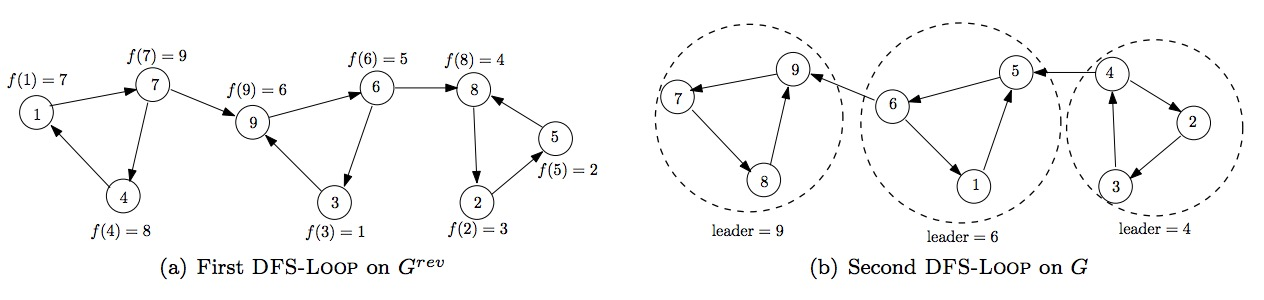
\includegraphics[width=\textwidth]{egscc.jpg}
\caption{Example of Algorithm \ref{twopassscc}}\label{egscc}
\end{figure}
\begin{algorithm}[ht]
\caption{Kosaraju's 2-Pass SCC Algorithm - DFS}\label{twopassscc}
\begin{algorithmic}[1]
\Input\Statex{Directed graph $G(V,E)$ with $n$ nodes labeled 1 to $n$}
\Output\Statex{SCCs of $G$}
\State{Reverse $G$ to get $G^{rev}$}
\State{\color{blue}1$^{st}$ loop: $DFSLoop(G^{rev})$}
\State{\color{red}2$^{nd}$ loop: $DFSLoop(G)$}
\Function{$DFSLoop$}{Graph $G$}
\State{Set all nodes unexplored}
\State{$t\coloneqq 0$, $s\coloneqq null$}\Comment{$t$: finish time. $s$: current leader}
\State{\color{red}2$^{nd}$ loop only: Relabel nodes according to $f(i)$}
\For{$i$ = $n$ \textbf{to} 1}
\If{$i$ not explored}
\State{\color{red}2$^{nd}$ loop only: $s\coloneqq i$}
\State{$DFS(G,i)$}
\EndIf
\EndFor
\EndFunction
\Function{$DFS$}{Graph $G$, node $i$}
\State{Mark $i$ as explored}
\State{\color{red}2$^{nd}$ loop only: $leader(i)\coloneqq s$}
\For{each arc $i\rightarrow j\in E$}
\If{$j$ not explored}
\State{$DFS(G,j)$}
\EndIf
\State{\color{blue}1$^{st}$ loop only: $f(i)\coloneqq ++t$}
\EndFor
\EndFunction
\end{algorithmic}
\end{algorithm}

The SCCs of a directed graph induce a meta-DAG. The meta-nodes are the SCCs, while its arcs are the original arcs between different SCCs, as shown in Figure \ref{metagraph}. It is guaranteed to be a DAG because the existence of any loop in the meta-graph will force a few SCCs to collapse into one big SCC.
\begin{figure}[ht]
\centering
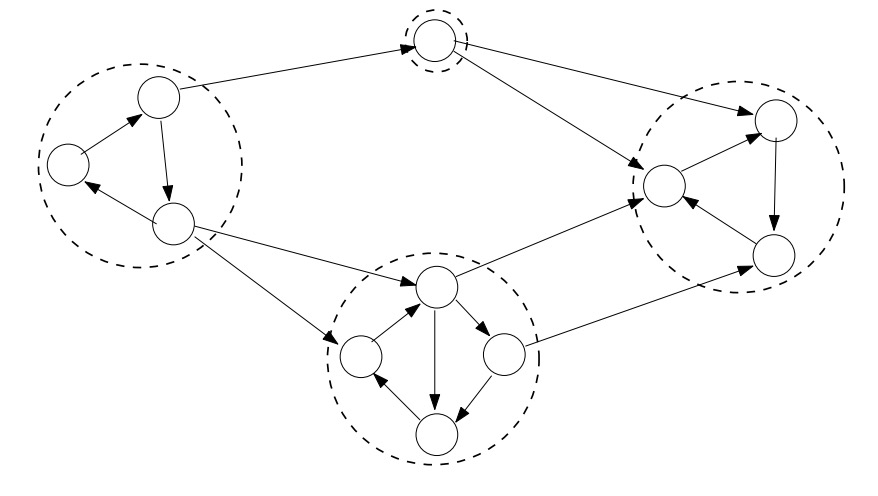
\includegraphics[width=0.5\textwidth]{metagraph.jpg}
\caption{Meta-graph induced by SCCs}\label{metagraph}
\end{figure}

DFS from a node is guaranteed to reach all other nodes in the same SCC, but it will also reach other SCCs as long as there exist outgoing arcs from this SCC, which are also outgoing arcs in the meta-DAG. Sink nodes in the meta-DAG do not have outgoing arcs, thus the correspondent SCC can be isolated if we start a DFS from one node in this SCC. Algorithm \ref{twopassscc} does exactly this. In order to prove its correctness we need the following lemma.
\begin{lemma}\label{keylemmascc}
Consider two adjacent SCCs of $G$: $C_1$ and $C_2$ such that $\exists$ arc $i\rightarrow j$ in which $i\in C_1,\:j\in C_2$. Let $f(v)$ denote the finishing time determined in the 1$^{st}$ loop of Algorithm \ref{twopassscc} for node $v$. Then we must have
$$\max\limits_{v\in C_1}f(v)<\max\limits_{v\in C_2}f(v).$$
\end{lemma}
\begin{proof}
In $G^{rev}$, there exists arc $j\rightarrow i$. Let $v$ represent the first vertex in $C_1\cup C_2$ to be explored. $v$ can be in either $C_1$ or $C_2$, as shown in Figure \ref{prooflemmascc}.
\begin{figure}[ht]
\centering
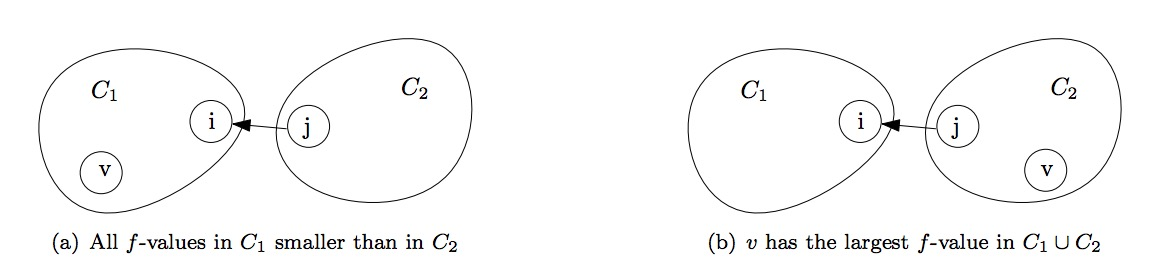
\includegraphics[width=\textwidth]{prooflemmascc.jpg}
\caption{Proof of Lemma \ref{keylemmascc}}\label{prooflemmascc}
\end{figure}

If $v\in C_1$, then none of the nodes in $C_2$ will be explored before all nodes in $C_1$ are explored, because there exists no arc from $C_1$ to $C_2$. Thus we have $f(v_1)<f(v_2),\:\forall v_1\in C_1, v_2\in C_2$, which is a stronger conclusion than our original argument in the lemma.

If $v\in C_2$, DFS for $v$ won't finish before DFSs for all nodes in $C_2$ finish. In particular, DFS for $j$ won't finish before DFS for all nodes in $C_1$ finish. Hence $v$ will have the largest $f$ value amongst all nodes in $C_1\cup C_2$, and we have $f(v)=\max\limits_{i\in C_2}f(i)>\max\limits_{i\in C_1}f(i)$ 
\end{proof}

An obvious corollary of Lemma \ref{keylemmascc} is as follow.
\begin{corollary}\label{corollaryscc}
$\max\limits_{v\in V}f(v)$ must lie in a sink SCC, i.e. an SCC that has no outgoing arc. 
\end{corollary}
Therefore, by starting from the node with the largest $f$ value in the 2$^{nd}$ loop, we are guaranteed to explore a sink SCC of $G$ first. Nodes in this sink SCC are ruled out from further exploration because there have been marked as explored. Every time we set up a new leader, it is guaranteed to be the node with the largest $f$ value amongst all unexplored nodes. DFS from the leader will reach and will only reach nodes in the same SCC as the leader, which is a sink SCC of the unexplored part of the graph. The SCCs will be found one by one.
\section{Dijkstra's Shortest Path Algorithm}
If all edges in a graph have equal lengths, the shortest path problem can be solved by BFS, as discussed in Algorithm \ref{shortestpath}. Dijkstra's algorithm computes shortest paths when edges have different lengths.
\begin{description}
\item[Input]Directed graph $G(V,E)$. Each edge $e\in E$ has non-negative length $l_e$. A source vertex $s$.
\item[Output]For each $v\in V$, compute the length of shortest path from $s$ to $v$ in $G$.
\end{description}
For convenience, we assume that there exists a path from $s$ to any vertex in $G$. 
\subsection{Algorithm}
Dijkstra's algorithm is shown in Algorithm \ref{dijkstra}.
\begin{algorithm}[ht]
\caption{Dijkstra's Shortest Path Algorithm}\label{dijkstra}
\begin{algorithmic}[1]
\Input\Statex{Directed graph $G(V,E)$. Each edge $e\in E$ has non-negative lengths $l_e$}
\Statex{Source vertex $s$}
\Output\Statex{Shortest path from $s$ to $v$ for all $v\in V$}
\State{Initialize $X=\{s\}$}\Comment{$X$: vertices processed so far}
\State{$A[s]=0$}\Comment{$A[v]$: length of shortest path from $s$ to $v$}
\State{$B[s]= empty\:path$}\Comment{$B[v]$: shortest path from $s$ to $v$}
\While{$X\neq V$}
\State{Among all edges $v\rightarrow w$ with $v\in X,w\notin X$, choose $v^*\rightarrow w^*$ that minimizes $A[v]+l_{vw}$}\Comment{Let's call it ``Dijkstra's greedy score''}
\State{$X\coloneqq X\cup\{w^*\}$}
\State{$A[w^*]\coloneqq A[v^*]+l_{v^*w^*}$}
\State{$B[w^*]\coloneqq B[v^*]+v*\rightarrow w^*$}
\EndWhile
\end{algorithmic}
\end{algorithm}
\subsection{Correctness}
The correctness of Dijkstra's algorithm can be proved by induction.
\begin{proof}
We will try to prove by induction that after each iteration,$\forall v\in X$, $B[v]$ is the shortest path from $s$ to $v$, and $A[v]$ is the length of the shortest path. 

At the beginning, $X=\{s\}$, $A[s]=0$, $B[s]=empty\:path$. Obviously the conclusion is correct. Let's assume that it holds before an iteration, and in this iteration we have chosen the edge $v^*\rightarrow w^*$. In order to add $w^*$ to $X$, we have to prove that $B[v^*]+v^*\rightarrow w^*$ with length $A[v^*]+l_{v^*w^*}$ is the shortest path from $s$ to $w^*$.

Take any path $S$ from $s$ to $w^*$. It has to cross the boundary between $X$ and $V-X$ somewhere. Suppose the edge from $X$ to $V-X$ is $y\rightarrow z$. This path can be divided into 3 segments:
\begin{enumerate}
\item $S_1$: from $s$ to $y$. According to our assumption, it is at least as long as $A[y]$: $L(S_1)\geq A[y]$.
\item $S_2$: the edge $y\rightarrow z$. $L(S_2)=l_{yz}.$
\item $S_3$: from $z$ to $w$. All edges have non-negative length, thus $L(S_3)\geq 0.$
\end{enumerate}
Dijkstra's algorithm guarantees that 
$$A[v^*]+l_{v^*w^*}\leq A[y]+l_{yz}.$$
Thus we have 
$$L(S)=L(S_1)+L(S_2)+L(S_3)\geq A[y]+l_{yz}\geq A[v^*]+l_{v^*w^*}.$$
Therefore, $B[v^*]+v^*\rightarrow w^*$ is the shortest path from $s$ to $w^*$.
\end{proof}
\subsection{Implementation and Running Time}
A naive implementation of Dijkstra's algorithm can take as long as $O(nm)$ time to run: in each iteration, we have to scan through all edges to find $v^*\rightarrow w^*$. In order to speed up the execution, we have to turn to the heap data structure.

Heap is a data structure designed to perform insertion and extraction of minimum in $O(\log n)$ time. Conceptually, a heap is an almost perfectly balanced binary tree (null leaves are only allowed at the lowest level). The key of each node must be smaller (or equal to) that of its two children. This property guarantees that the node with the smallest key is at the root. Insertion is performed by adding the element behind the last node and bubbling up, while extraction of minimum is performed by swapping the root and the last node and then bubbling down. The height of the tree is $O(\log n)$, thus insertion and extraction of minimum can be executed in $O(\log n)$ time. 

In the implementation of Dijkstra's algorithm, we use a heap to store the vertices in $V-X$. The key of a node is the smallest Dijkstra's greedy score related to this vertex, i.e. for $v\in V-X$, $key[v]$ is the smallest value of $A[u]+l_{uv},\forall u\in X$. If such edge $u\rightarrow v$ does not exist, $key[v]=+\infty.$ In each iteration of Dijkstra's algorithm, we extract the minimum of the heap and denote it with $w$. Now we should have $w\in X$, and $A[w]$ is the length of the shortest path from $s$ to $w$. Then for all edges $w\rightarrow v$ with $v\in V-X$, we update the key of $v$:
$$key[v]\coloneqq\min\{A[w]+l_{wv},key[v]\}.$$
If $key[v]$ is changed here, we bubble it down in the heap, which is a $O(\log n)$ operation. In this way the heap gets maintained at each iteration.

In total, we do $n-1$ extractions of minimum, and at most $m$ bubbling down of element in the heap. Each of these operations is $O(\log n)$, thus the total time consumption is $O((m+n)\log n)$. Since the graph is weakly connected ($\forall v\exists$ path from $s$ to $v$), we have $m\geq n-1$, hence $O(m+n)=O(m)$. In conclusion, the running time of Dijkstra's algorithm implemented using heap is $O(m\log n)$.
\ifx\PREAMBLE\undefined
\end{document}
\fi